%#######################################################################
%
% Introduction and motivation for open tool support and VDM + UML
%
\section{Connecting UML and VDM++}
%-----------------------------------------------------------------------
%
% Outline
%
\begin{frame}
  \frametitle{Outline}
  \tableofcontents[current]
\end{frame}


%-----------------------------------------------------------------------
\subsection{History}
%-----------------------------------------------------------------------
%
% VDM Tools
%
%\frame
%{
%  \frametitle{Existing tool}
%
%VDM Tools
%  \begin{itemize}
%	%\itemsep=1cm
%  		\item<1-> Commercial tool from CSK
%  		\item<2-> No editor
%  		\item<3-> Includes a UML transformation
%  		\begin{itemize}
%  			\item Rose VDM Link first release (1997)
%  			\item UML 1.4
%  		\end{itemize}
%	  	
%  \end{itemize}
%
%
%}
%
%
%\note
%{
%
%  \begin{itemize}
%	%\itemsep=1cm
%  		\item Only tool
%  		\item Commercial
%  		\item Older UML Transformation Rose VDM Link from (1997)
%  		\item UML 1.4
%	  	
%  \end{itemize}
%
%
%
%
%}


%-----------------------------------------------------------------------
\subsection{Using Sequence diagrams for test automation}
%-----------------------------------------------------------------------

%
% extending uml trans
%
%\frame
%{
%  \frametitle{Extending UML support}
%
%  \begin{itemize}
%	\itemsep=1cm
%  		\item<1-> Change to UML version 2.x
%  		\item<2-> Extend UML subset for Class Diagrams
%  		\item<3-> UML Sequence Diagrams
%	  	
%  \end{itemize}
%
%
%}
%
%\note
%{
%
%  \begin{itemize}
%	%\itemsep=1cm
%  		\item Since UML 2 has since been released look into new features and uses
%  		\item Extending the subset of UML used to model VDM, active, abstract,x-or association
%  		\item Look into new diagrams which could be use full, new VDM feature for testing \textbf{Traces}
%	  	
%  \end{itemize}
%
%}


%
% Traces
%
%\frame
%{
%  \frametitle{Combinatorial Testing in VDM}
%
%  \begin{itemize}
%	%\itemsep=1cm
%  		\item<1-> New feature recently introduced to VDM - 2008
%  		\item<2-> Automatic execution of a large number of test cases generated from templates in form of trace definitions
%  		\item<3-> Add graphical representation of trace definitions in UML as Sequence Diagrams
%	  	
%  \end{itemize}
%
%
%}

%
% Traces example
%
%\frame
%{
%  \frametitle{VDM Combinatorial Test example}
%\begin{center}
%\vdmSpecLineNum{UseStack.vpp}{Traces}{VDM:Collections}
%
%\end{center}
%}



%
% Traces example expanded
%
\begin{frame}[fragile] 

  \frametitle{VDM Combinatorial Test example evaluation}
\begin{columns}
\begin{column}[l]{5cm}

%\begin{itemize}\footnotesize
%\item Set selection \tikz\node [fill=blue!20,draw,circle] (n1) {};
%\item Repeat \tikz\node [fill=red!20,draw,circle] (n2) {};
%\end{itemize}

	\begin{center}
\onslide<2->{ 
\begin{tikzpicture}
[
	overlay,
	xscale	= 1,	% to scale horizontally everything but the text
	yscale	= 1,	% to scale vertically everything but the text
]
	\node[fill=blue!20,text height=0.2ex,text width=2ex, text depth=0.25ex]	at	(1.2,-1.7) (t1){ };

	\node[fill=red!20,text height=0.2ex,text width=2ex, text depth=0.25ex]	at	(1.8,-2.5) (t1){ };

	\node[fill=green!20,text height=0.2ex,text width=0.5ex, text depth=0.25ex]	at	(-0.6,-3.7) (t1){ };
\end{tikzpicture}
}
	\vdmSpecLineNum{UseStackTrace.vpp}{Traces}{VDM:Collections}
	\end{center}

\end{column}
\begin{column}[r]{5cm}
	\begin{itemize}
		\item<3-> TC1:
		\begin{itemize}
			\item stack.Reset()
			\item stack.Push(2)
			\item stack.Push(5)
		\end{itemize}
		\item<4-> TC2:
		\begin{itemize}
			\item stack.Reset()
			\item stack.Push(8)
			\item stack.Push(8)
			\item stack.Pop()
		\end{itemize}
		\item<5-> ... 14 more
	\end{itemize}



\end{column}
\end{columns}
\end{frame}
\note{
show x in set (2,8)
show {1,4} repeat
show choice |

}


\frame
{
  \frametitle{Combinatorial Test form Overture}
	\begin{center}
	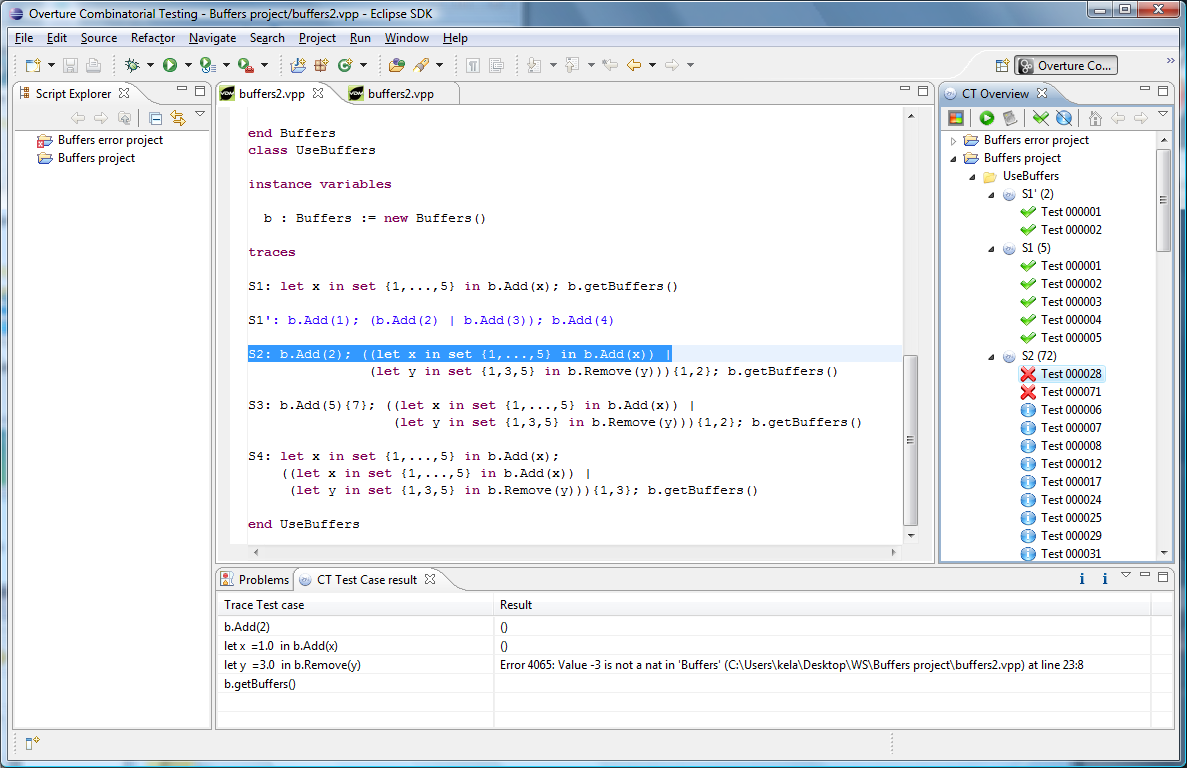
\includegraphics[width=0.9\textwidth]{images/CTOverview.png}%
	\end{center}
}

%
% Traces example UML
%
\frame
{
  \frametitle{VDM Combinatorial Test example Sequence Diagram}
  
\begin{columns}
\begin{column}[l]{5cm}

	\begin{center}
	\vdmSpecLineNum{UseStackTrace.vpp}{Traces}{VDM:Collections}
	\end{center}

\end{column}
\begin{column}[r]{5cm}
	
	\begin{center}
	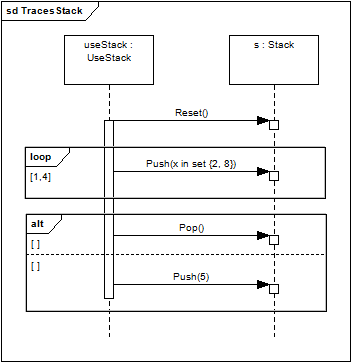
\includegraphics[width=\textwidth]{images/TracesSequenceDiagramEx2.png}%
	\end{center}

\end{column}
\end{columns}
  

}

